% ============================================================
%  SCHOLA DOMESTICA — Magister Mathematica
%  Level 1 | Week 7 | Day 2
%  Topic: Addition — Joining Groups (0+n, small sums, pictures)
%  +0, +1, +2 mixed; number line jumps; writing addition sentences
% ============================================================
\documentclass[12pt, letterpaper]{article}

\usepackage[top=1in, bottom=1in, left=1in, right=1in]{geometry}
\usepackage{fontenc}
\usepackage{inputenc}
\usepackage{lmodern}
\usepackage{microtype}
\usepackage{amsmath}
\usepackage{graphicx}
\usepackage{xcolor}
\usepackage{tikz}
\usepackage{array}
\usepackage{enumitem}
\usepackage{multicol}
\usepackage{mdframed}
\usepackage{fancyhdr}

\definecolor{scholared}{RGB}{160,30,30}
\definecolor{scholagold}{RGB}{180,140,40}
\definecolor{scholacream}{RGB}{253,248,235}
\definecolor{scholagreen}{RGB}{50,110,60}
\definecolor{scholablue}{RGB}{40,80,140}

\pagestyle{fancy}
\fancyhf{}
\renewcommand{\headrulewidth}{0.6pt}
\fancyhead[L]{\small\textcolor{scholared}{\textbf{Schola Domestica — Magister Mathematica}}}
\fancyhead[R]{\small\textcolor{scholared}{Level 1 · Week 7 · Day 2}}
\fancyfoot[C]{\small\textcolor{gray}{— \thepage\ —}}

\newcommand{\answerline}{\underline{\hspace{2.5cm}}}
\newcommand{\biganswerline}{\underline{\hspace{4cm}}}
\newcommand{\numbox}{\fbox{\hspace{0.6cm}\vphantom{0}}}

\newmdenv[
  backgroundcolor=scholacream,
  linecolor=scholared,
  linewidth=1.5pt,
  roundcorner=6pt,
  innertopmargin=8pt,
  innerbottommargin=8pt,
  innerleftmargin=10pt,
  innerrightmargin=10pt
]{lessonbox}

\begin{document}

\begin{center}
  {\LARGE\textbf{\textcolor{scholared}{Addition: +0, +1, +2}}}\\[4pt]
  {\Large\textcolor{scholagold}{\textit{Number Line Jumps and Addition Sentences}}}\\[6pt]
  {\small Name: \biganswerline \hspace{1cm} Date: \answerline}
\end{center}

\vspace{4pt}
\noindent\textcolor{scholared}{\rule{\linewidth}{1pt}}
\vspace{4pt}

% IMAGE PROMPT (Beatrix Potter watercolour style):
% A small hedgehog collecting mushrooms in an autumn forest. He has a basket with 4 mushrooms;
% two more mushrooms stand nearby. The hedgehog looks at them happily. Warm amber and
% ochre watercolour tones. No text.

\begin{lessonbox}
\textbf{Adding Zero:} When you add \textbf{0} (nothing), the number stays the same.\\[4pt]
$6 + 0 = 6$ \quad $9 + 0 = 9$ \quad $0 + 7 = 7$\\[6pt]
\textbf{The number line} shows addition as \textbf{hops forward}.\\
$5 + 2$: start at 5, hop forward 2 times — land on \textbf{7}.
\end{lessonbox}

\bigskip

% ===== PART I: NUMBER LINE ADDITION =====
\noindent\textcolor{scholared}{\large\textbf{Part I — Number Line Hops}} \hfill \textit{(Problems 1–4)}

\begin{center}
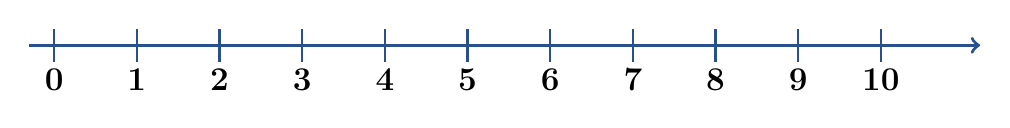
\begin{tikzpicture}[scale=1.05]
  \draw[very thick, scholablue, ->] (-0.3,0) -- (11.2,0);
  \foreach \n in {0,...,10} {
    \draw[thick, scholablue] (\n,0.2) -- (\n,-0.2);
    \node[below=5pt] at (\n,0) {\large\textbf{\n}};
  }
\end{tikzpicture}
\end{center}

\bigskip
\noindent\textbf{1.} Draw jumps on the number line for $6 + 2$. Answer: \hfill \answerline

\bigskip
\noindent\textbf{2.} Draw jumps on the number line for $7 + 1$. Answer: \hfill \answerline

\bigskip
\noindent\textbf{3.} Draw jumps on the number line for $5 + 2$. Answer: \hfill \answerline

\bigskip
\noindent\textbf{4.} Draw jumps on the number line for $8 + 0$. Answer: \hfill \answerline

\bigskip
\noindent\textcolor{scholared}{\rule{\linewidth}{0.4pt}}

% ===== PART II: WRITE THE ADDITION SENTENCE =====
\noindent\textcolor{scholared}{\large\textbf{Part II — Write the Addition Sentence}} \hfill \textit{(Problems 5–8)}

\medskip
\noindent\textit{Count each group. Write the addition sentence and the sum.}

\bigskip
\noindent\textbf{5.} \quad

\begin{tikzpicture}[baseline=-0.5ex]
  \foreach \i in {1,...,5}{\filldraw[scholablue](\i*0.38,0)circle(0.13cm);}
\end{tikzpicture}
\quad and \quad

\begin{tikzpicture}[baseline=-0.5ex]
  \foreach \i in {1,...,2}{\filldraw[scholared](\i*0.38,0)circle(0.13cm);}
\end{tikzpicture}

\medskip
\hspace{2em} \numbox \; $+$ \; \numbox \; $=$ \; \numbox

\bigskip
\noindent\textbf{6.} \quad

\begin{tikzpicture}[baseline=-0.5ex]
  \foreach \i in {1,...,7}{\filldraw[scholagreen](\i*0.38,0)circle(0.13cm);}
\end{tikzpicture}
\quad and \quad

\begin{tikzpicture}[baseline=-0.5ex]
  \foreach \i in {1,...,1}{\filldraw[scholagold](\i*0.38,0)circle(0.13cm);}
\end{tikzpicture}

\medskip
\hspace{2em} \numbox \; $+$ \; \numbox \; $=$ \; \numbox

\bigskip
\noindent\textbf{7.} \quad

\begin{tikzpicture}[baseline=-0.5ex]
  \foreach \i in {1,...,4}{\filldraw[scholared](\i*0.38,0)circle(0.13cm);}
\end{tikzpicture}
\quad and \quad

\begin{tikzpicture}[baseline=-0.5ex]
  \foreach \i in {1,...,0}{\filldraw[scholablue](\i*0.38,0)circle(0.13cm);}
\end{tikzpicture}
\textit{(no dots)}

\medskip
\hspace{2em} \numbox \; $+$ \; $0$ \; $=$ \; \numbox

\bigskip
\noindent\textbf{8.} \quad

\begin{tikzpicture}[baseline=-0.5ex]
  \foreach \i in {1,...,6}{\filldraw[scholablue](\i*0.38,0)circle(0.13cm);}
\end{tikzpicture}
\quad and \quad

\begin{tikzpicture}[baseline=-0.5ex]
  \foreach \i in {1,...,2}{\filldraw[scholared](\i*0.38,0)circle(0.13cm);}
\end{tikzpicture}

\medskip
\hspace{2em} \numbox \; $+$ \; \numbox \; $=$ \; \numbox

\bigskip
\noindent\textcolor{scholared}{\rule{\linewidth}{0.4pt}}

% ===== PART III: QUICK FACTS =====
\noindent\textcolor{scholared}{\large\textbf{Part III — Quick Facts}} \hfill \textit{(Problems 9–12)}

\bigskip
\begin{multicols}{2}
\noindent\textbf{9.} $\; 3 + 0 = $ \numbox \\[12pt]
\noindent\textbf{10.} $\; 5 + 1 = $ \numbox \\

\columnbreak

\noindent\textbf{11.} $\; 0 + 8 = $ \numbox \\[12pt]
\noindent\textbf{12.} $\; 6 + 2 = $ \numbox \\
\end{multicols}

\end{document}
